% -*- program: xelatex -*-
\documentclass[11pt]{beamer} 
%\usepackage{beamerthemesplit}

\usepackage{fontspec}
\setsansfont{PT Sans}
\setmonofont{PT Mono}
\usepackage{pgfpages}
\usepackage{mathabx}

\usepackage{beamerthemesplit}
\usefonttheme[onlymath]{serif}

\usetheme{CambridgeUS}
\usecolortheme{lily}

\hypersetup{unicode=true}
\DeclareFontEncoding{T1}
\fontencoding{T1} 
\usepackage[russian]{babel}

\usepackage{amsmath,amssymb,amsthm}
\usepackage{unicode-math}
\usepackage{xltxtra}
\setmathfont{Asana Math}

\usepackage{graphics,graphicx}
\usepackage{listings}
\usepackage{media9}
\usepackage{verbatim}
\usepackage{fancyvrb}
\usepackage{booktabs}
\usepackage{colortbl}
\usepackage{multirow}
\usepackage{verbatim}
\usepackage{fancyvrb}
\usepackage{color}

\newtheorem{ru_def}{Теорема}
\renewenvironment{theorem}{\begin{ru_def}}{\end{ru_def}}

\definecolor{mygreen}{RGB}{28,172,0} % color values Red, Green, Blue
\definecolor{mylilas}{RGB}{170,55,241}
\definecolor{codecolor}{RGB}{0,120,0}
\definecolor{light-gray}{gray}{0.95}
\definecolor{light-green}{RGB}{205,255,204}
\definecolor{light-red}{rgb}{0.9, 0.8, 0.8}
\definecolor{light-yellow}{rgb}{1,1,0.85}
\definecolor{light-blue}{RGB}{255,204,153}
\definecolor{dark-blue}{rgb}{0,0,0.6}
\definecolor{dark-red}{RGB}{204,0,0}
\definecolor{dark-green}{RGB}{28,172,0}

\usepackage{pifont}% http://ctan.org/pkg/pifont
\newcommand{\cmark}{\textcolor{green}{\ding{51}}}
\newcommand{\xmark}{\textcolor{red}{\ding{55}}}

\setbeamercolor{frametitle}{fg=dark-red,bg=gray!10}
\setbeamerfont{title}{series=\bfseries,parent=structure}
\setbeamerfont{frametitle}{series=\bfseries,parent=structure}
\setbeamertemplate{blocks}[rounded][shadow=false]
\setbeamercolor{block title}{fg=structure,bg=white}
\setbeamertemplate{navigation symbols}{}

\renewcommand{\emph}[1]{\textcolor{dark-blue}{#1}}
\newcommand{\emphb}[1]{\textcolor{dark-blue}{\textbf{#1}}}

\usepackage{tikz}
\usetikzlibrary{arrows,matrix,positioning}

%\warn{\matcode}[1]{ \textcolor{codecolor}{\texttt{#1}}}
%\newcommand{\matcode}[1]{\begin{Verbatim}[formatcom=\color{red}]#1\end{Verbatim}}
\definecolor{codecolor}{RGB}{0,150,0}
\newcommand{\matcode}[1]{ \textcolor{codecolor}{\texttt{#1}}}


%\pgfdeclareimage[height=1cm]{logo}{ssau.pdf}
%\logo{\pgfuseimage{logo}}
%\setbeameroption{show notes}
%\graphicspath{{img/}}

\lstset{language=matlab, 
    keepspaces=true,
    extendedchars=true,
    basicstyle={\footnotesize  \color{black}},
    breaklines=true,
    morekeywords={matlab2tikz},
    keywordstyle=\color{blue},
    morekeywords=[2]{1}, keywordstyle=[2]{\color{codecolor}},
    identifierstyle={ \bf \color{black} },
    stringstyle=\color{mylilas},
    commentstyle=\color{mygreen},%
    showstringspaces=false,
    numbers=left,%
    numberstyle={\tiny \color{black}},
    numbersep=7pt, 
    emph=[1]{case,switch,otherwise},emphstyle=[1]\color{blue}, 
    frame=single,    
    %lineskip=-1.0pt,
    %emph=[2]{word1,word2}, emphstyle=[2]{style},    
}

\makeatother
\setbeamertemplate{footline}
{
  \leavevmode%
  \hbox{%  
  \begin{beamercolorbox}[wd=.3\paperwidth,ht=2.25ex,dp=1ex,center]{author in head/foot}%
    \usebeamerfont{author in head/foot}\insertshortauthor
  \end{beamercolorbox}%  
  \begin{beamercolorbox}[wd=.6\paperwidth,ht=2.25ex,dp=1ex,center]{title in head/foot}%
    \usebeamerfont{title in head/foot}\insertshorttitle
  \end{beamercolorbox}%
  \begin{beamercolorbox}[wd=.1\paperwidth,ht=2.25ex,dp=1ex,center]{date in head/foot}%
    \insertframenumber{} / \inserttotalframenumber\hspace*{1ex}
  \end{beamercolorbox}}%
  \vskip0pt%
}

\setbeamertemplate{headline}{}
%\setbeamertemplate{footline}{}

\AtBeginSection[]{
  \begin{frame}[plain]
  %\vfill  
  \begin{tikzpicture}
  \useasboundingbox (0,0) rectangle(\the\paperwidth,\the\paperheight);  
  \fill[color=dark-red]   (-1cm, 3.9cm) rectangle(\the\paperwidth, 5.9cm);
  %\usebeamerfont{title}\insertsectionhead\par%
  %\node[text width=\the\paperwidth,align=center] at (current page.center) {\color{ExecusharesWhite}\Large\textbf{\insertsectionhead}};  
  \node[text width=\the\paperwidth,align=center] at (6cm,4.9cm) {\color{white}\Large\textbf{\insertsectionhead}};  
  \end{tikzpicture}
  \end{frame}
}

\title{Относительное орбитальное движение}
%\subtitle{Компьютерный практикум по механике}
\author{Юдинцев В. В.}
\small
\institute{Кафедра теоретической механики}
 
\begin{document}

{
\usebackgroundtemplate{
\includegraphics[width=\paperwidth,height=\paperheight]{./back.png}}
\begin{frame}[plain]
\maketitle
\end{frame}
} 

\frame{
\frametitle{Содержание}
\tableofcontents
}


\begin{frame}[c]
\frametitle{Относительное движение}
\begin{itemize}
	\item Космическая станция движется по круговой орбите радиусом $r_0$
	\item Рассматривается движение объекта (КА или космонавта) относительно станции
	\item Предполагается, что расстояние между станцией и объектом $\rho$ намного меньше радиуса $r_0$ орбиты станции:
	$$
		\rho \ll r_0
	$$
	\item Движение объекта относительно станции рассматривается относительно \emph{орбитальной подвижной} системы координат $Ox_0y_0z_0$, \emph{движущейся со станцией}
\end{itemize}
\end{frame}
 
{
\usebackgroundtemplate{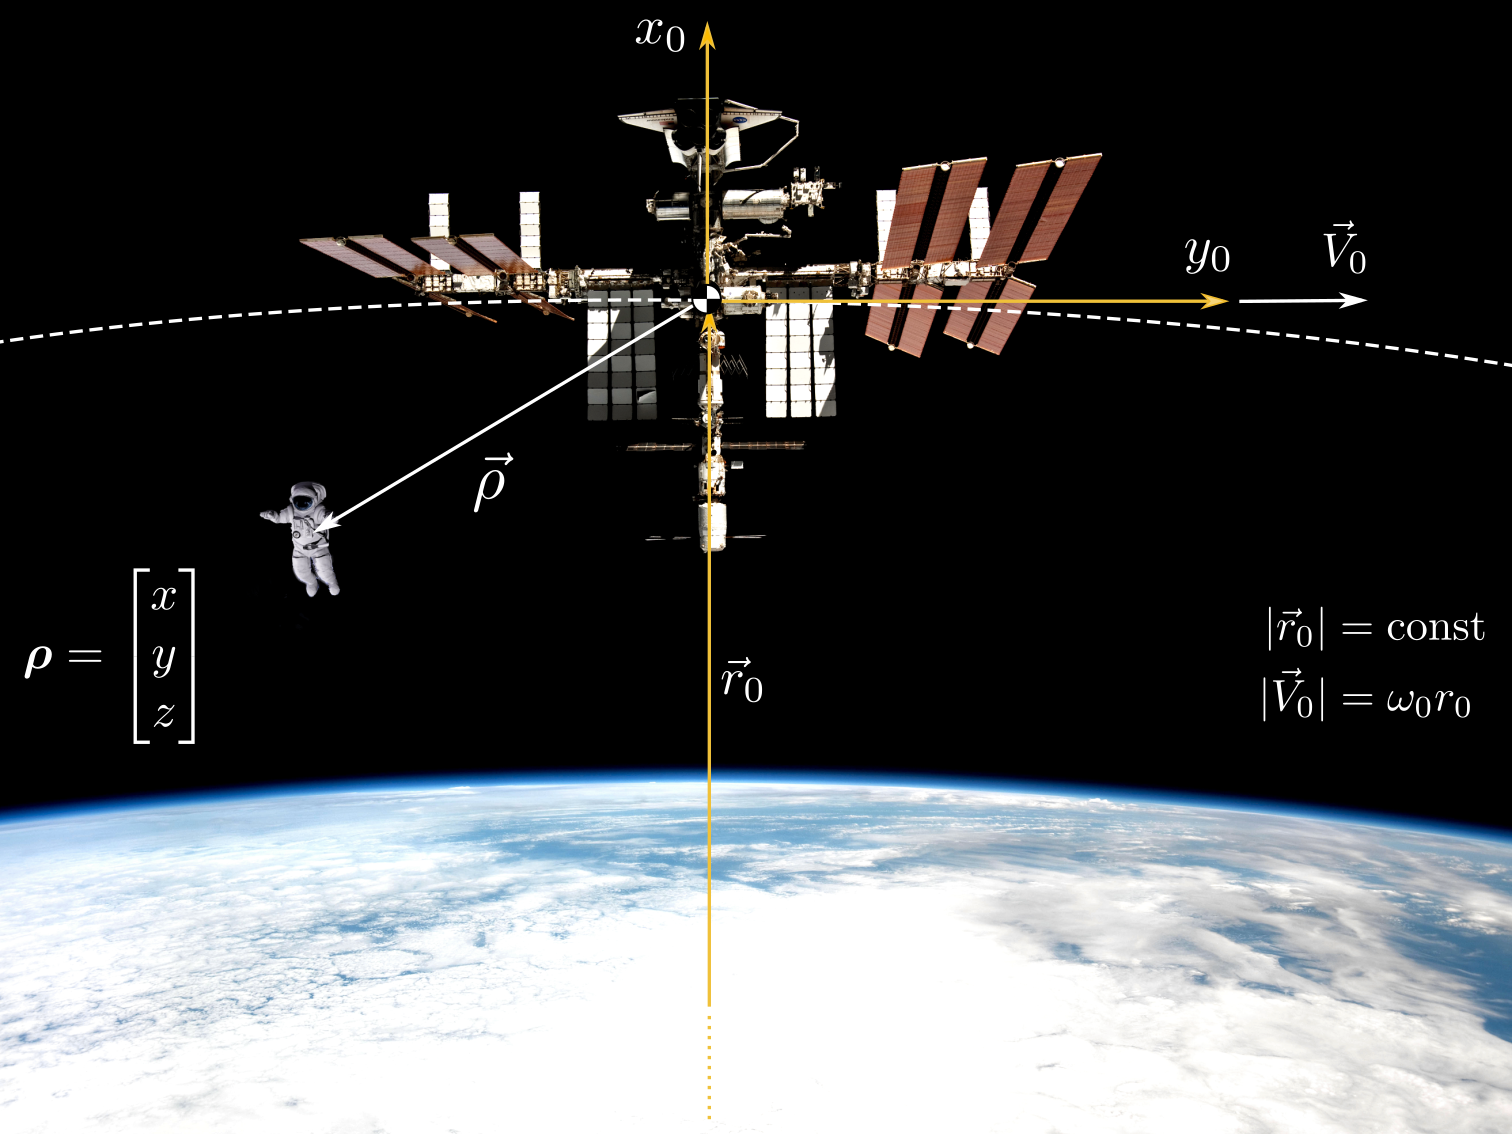
\includegraphics[width=\paperwidth,height=\paperheight]{./ManInSpace.png}}
\begin{frame}[plain]
\end{frame}
}

{
\usebackgroundtemplate{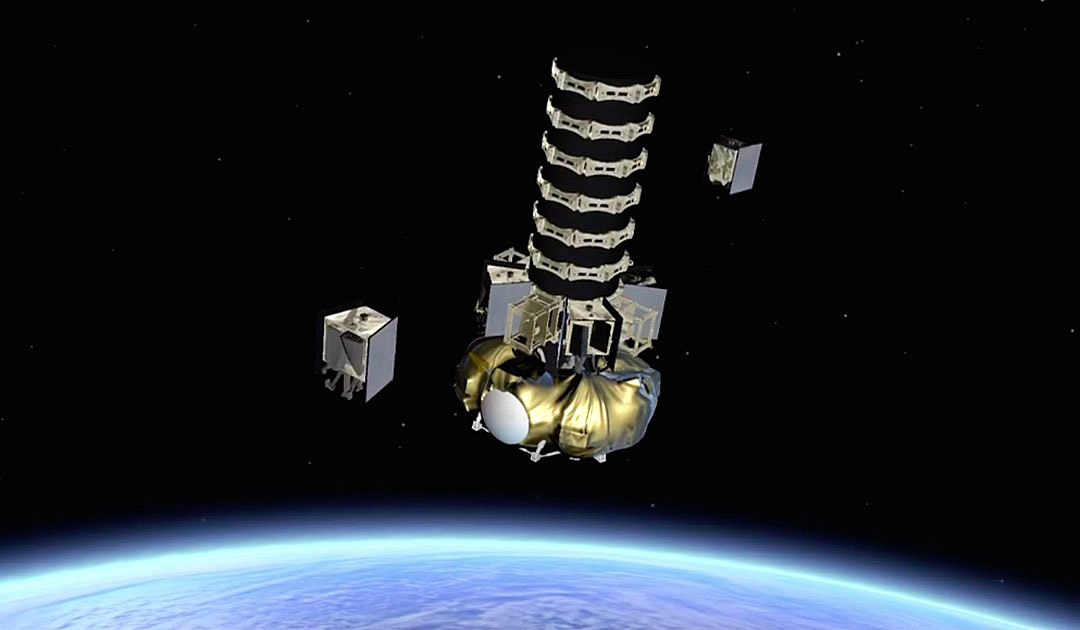
\includegraphics[width=\paperwidth,height=\paperheight]{./cluster.jpeg}}
\begin{frame}[plain]
\end{frame}
}

{
\usebackgroundtemplate{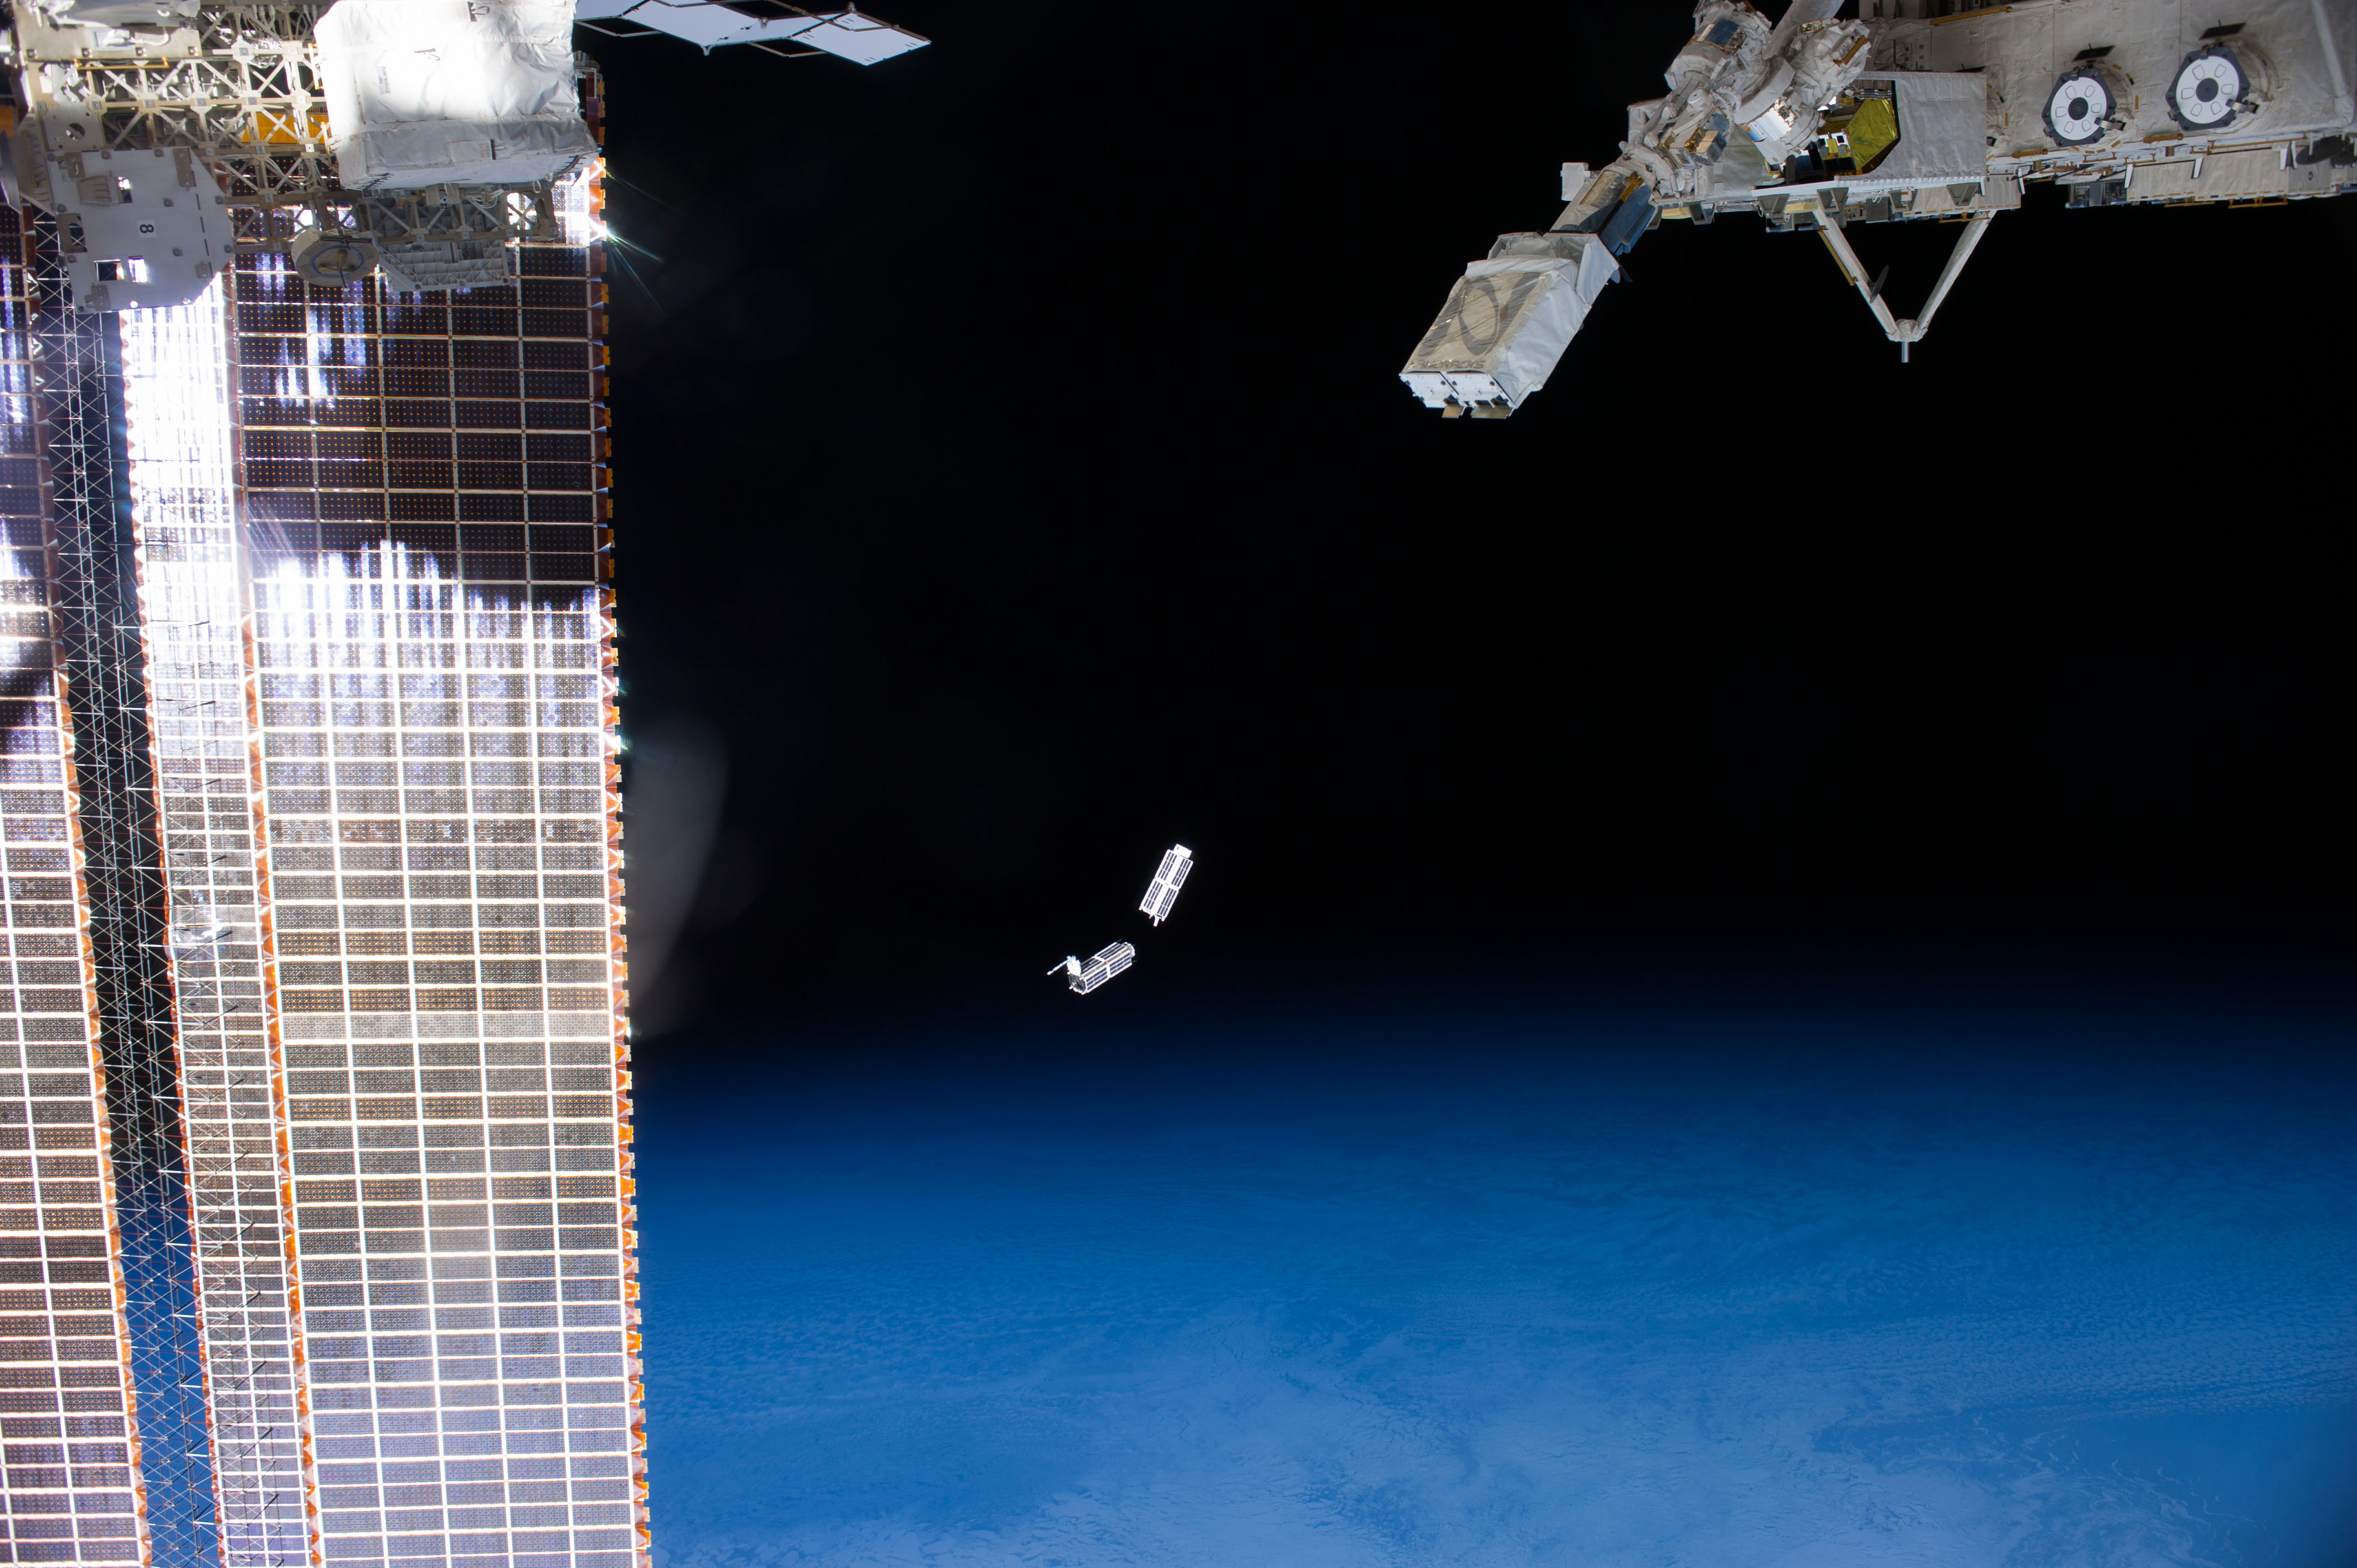
\includegraphics[width=\paperwidth,height=\paperheight]{./nanoracks.jpeg}}
\begin{frame}[plain]
\end{frame}
}

{
\usebackgroundtemplate{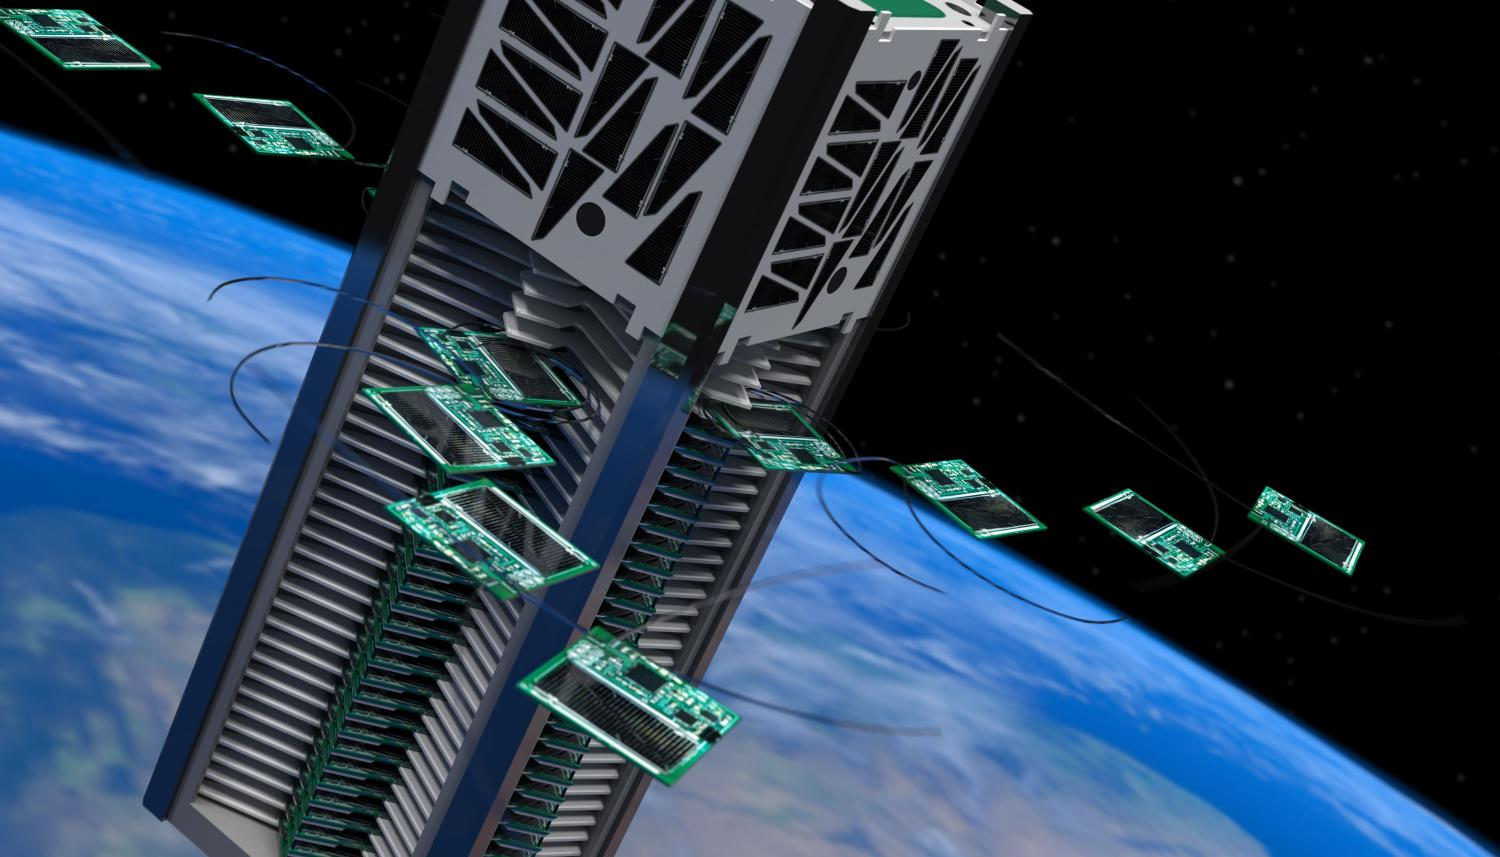
\includegraphics[width=\paperwidth,height=\paperheight]{./pico.jpeg}}
\begin{frame}[plain]
\end{frame}
}


\section{Орбитальная подвижная система координат} 

\frame{
\frametitle{Направление осей СК  $Ox_0y_0z_0$}
\begin{center}
 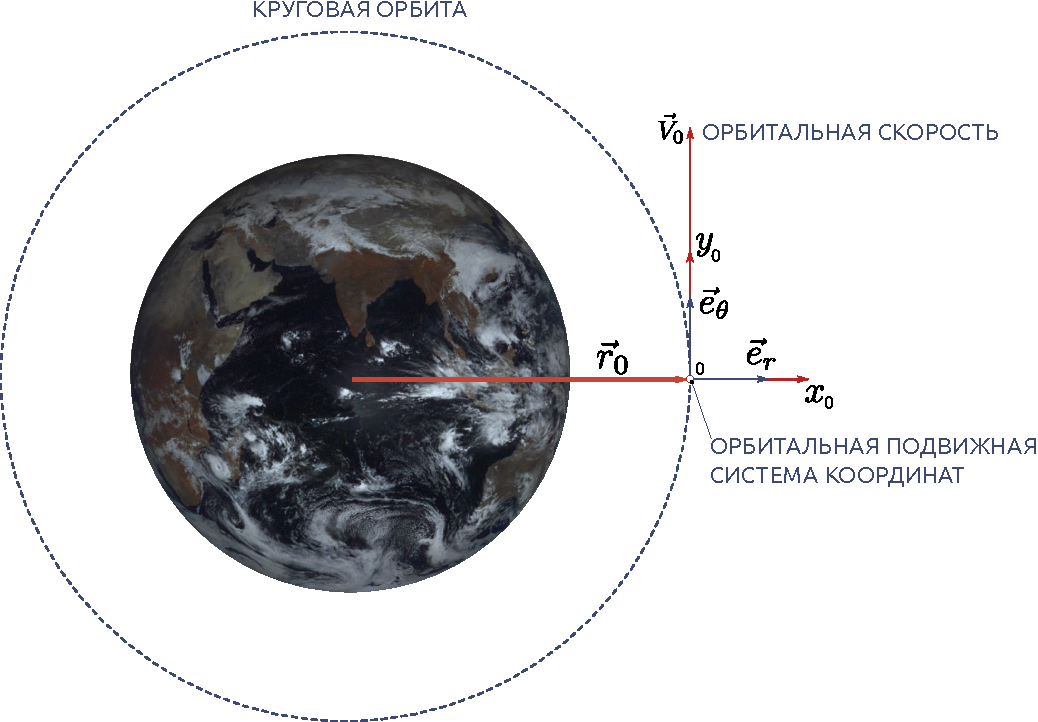
\includegraphics[width=1\linewidth]{./Orbital_SC.pdf}
\end{center}
}

\begin{frame}[c]
	\frametitle{Орбитальная подвижная система координат}  
	Направления осей орбитальной подвижной системы координат, связанной со станцией:
	\begin{itemize}
		\item $Ox_0$ -- направлена вдоль радиус-вектора центра масс станции относительно центра Земли
		\item $Oy_0$ -- направлена вдоль вектора орбитальной скорости станции
		\item $Oz_0$ -- направлена перпендикулярно плоскости орбиты
	\end{itemize}
	Положение объекта относительно системы координат $Ox_0y_0z_0$ определяется вектором $\vec \rho$. Орбитальная подвижная система координат является неинерциальной.
\end{frame}

\section{Движение станции}

\frame
{
\frametitle{Неинерциальная СК}
\begin{columns}
\column{0.4\linewidth}
\begin{center}
 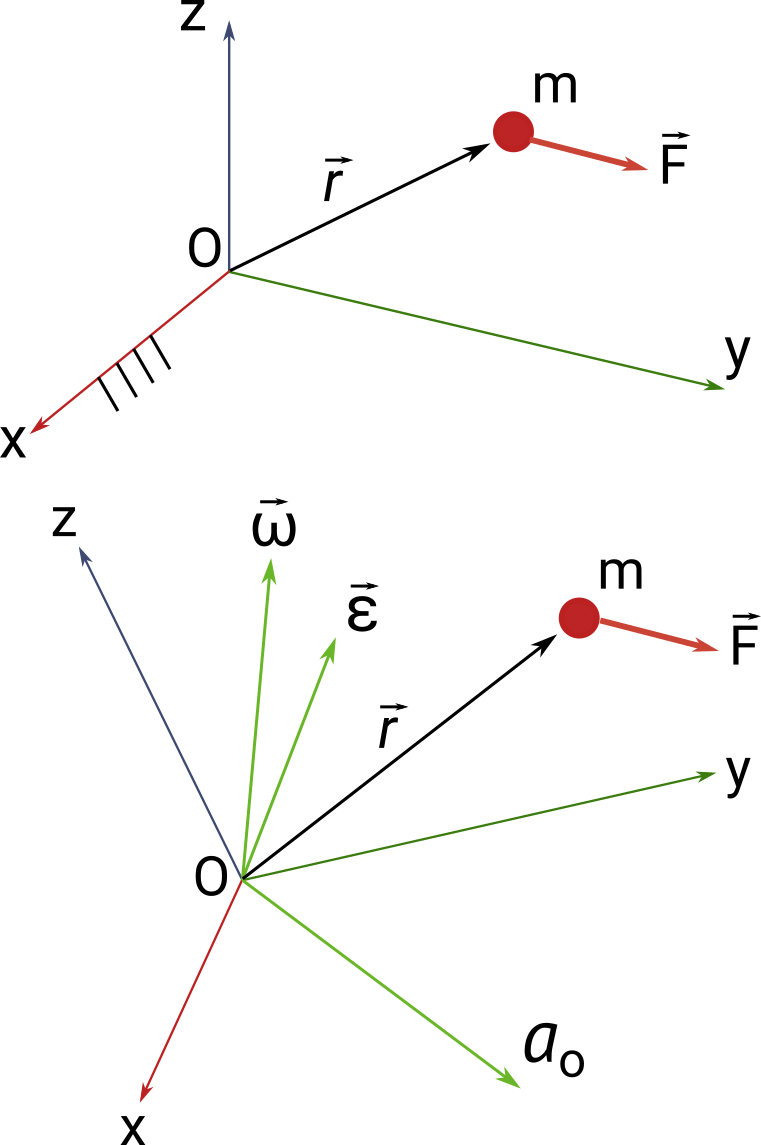
\includegraphics[width=1.0\linewidth]{noninertial_eq.png}
\end{center} 
\column{0.6\linewidth}
В инерциальной системе координат
\begin{equation}
	m \ddot{\vec{r}} = \vec F 
\end{equation}
В неинерциальной системе координат к активным силам добавляются <<силы инерции>>
\begin{equation}
	m \ddot{\vec{r}} = \vec F + \vec F_e + \vec F_c
\end{equation}
$$
\vec F_e = - m(\vec a_o + \vec \varepsilon \times \vec r + \vec \omega \times (\vec \omega \times \vec r)))
$$
$$
\vec F_c = - 2 m \left( \vec \omega \times \frac{\tilde{d}\,\vec r}{dt} \right)
$$
\end{columns}
}



\frame{
\frametitle{Скорость движения по орбите}
\alert{Система координат $Ox_0y_0z_0$ неинерциальная}. Ускорение  центра масс станции при её движении по круговой орбите с постоянной скоростью:
\begin{equation}
	a_0 = \frac{V_0^{2}}{r_0} = \omega_0^2 r_0	
\end{equation}
Это ускорение вызвано действием силы притяжения Земли:
\begin{equation}
	a_0 = \frac{F}{m} = \frac{\mu}{r_0^2}	
\end{equation}

} 


\frame{
\frametitle{Скорость движения по орбите}
Из равенства
\begin{equation}
	\omega_0^2 r_0 = \frac{\mu}{r_0^2}
\end{equation}
следует выражение для угловой скорости движения по орбите
\begin{equation}
 \omega_0 = \sqrt{\frac{\mu}{r_o^3}}
\end{equation}
и линейная скорость движения по орбите
\begin{equation}
V_0 = \omega_0 r_0 = \sqrt{\frac{\mu}{r_0}}
\end{equation}
Для орбиты высотой 500 км $r_0 = R_\Earth + 500$ км, $V_0 = 7788$ м/с, $\omega_0 = 0.001185$ рад/c 
} 



\frame{
\frametitle{Скорость движения по орбите}
Период обращения по круговой орбите высотой $h_0$
\begin{equation}
 T = \frac{2 \pi}{\omega_0} = 2 \pi \sqrt{\frac{r_o^3}{\mu}} = 2 \pi \sqrt{\frac{(R_\Earth+h_0)^3}{\mu}}
\end{equation}

Для круговой орбиты $h_0=500$ км:  T = 5668 с = 94 минуты.

Для круговой орбиты $h_0=200$ км:  T = 5301 с = 88 минут.
 
} 

\section{Уравнения относительного движения}


\frame
{
\frametitle{Уравнение относительного движения КА}
\begin{columns}
\column{0.6\linewidth}
\begin{center}
 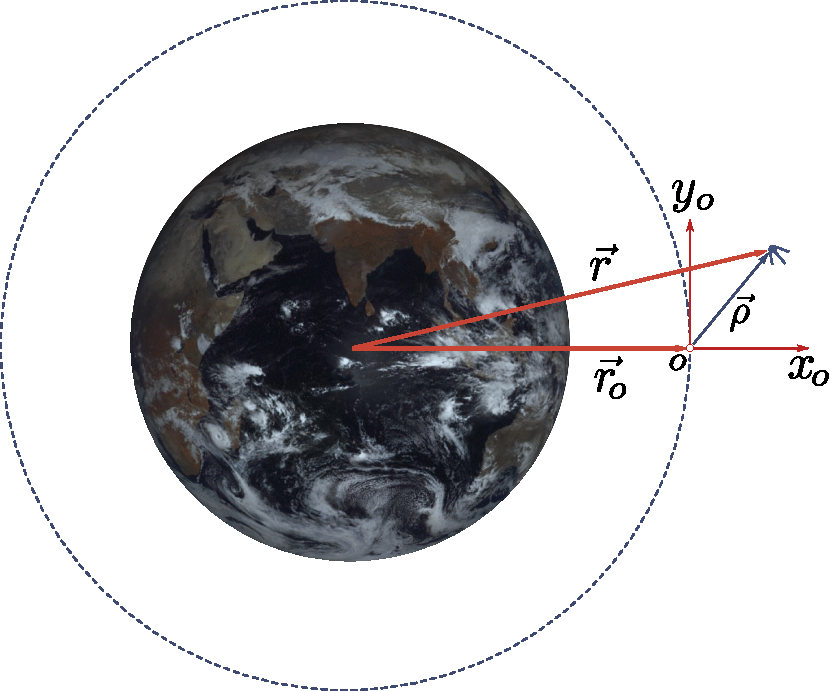
\includegraphics[width=1.0\linewidth]{./Orbital_SC_rho.pdf}
\end{center} 
\column{0.4\linewidth}
\begin{equation}
	\boxed{m \ddot{\vec{\rho}} = \vec F + \vec F_e + \vec F_c}	
\end{equation}
\begin{itemize}
 \item $\vec F_e$ -- переносная сила инерции
 \item $\vec F_c$ -- сила инерции Кориолиса
 \item $\vec F$ -- гравитационная сила
\end{itemize}
\end{columns}
}



\frame{
\frametitle{$Ox_0y_0z_0$ -- неинерциальная СК}
\begin{columns}
\column{0.4\linewidth}
\begin{figure}[htbp]
  \centering
  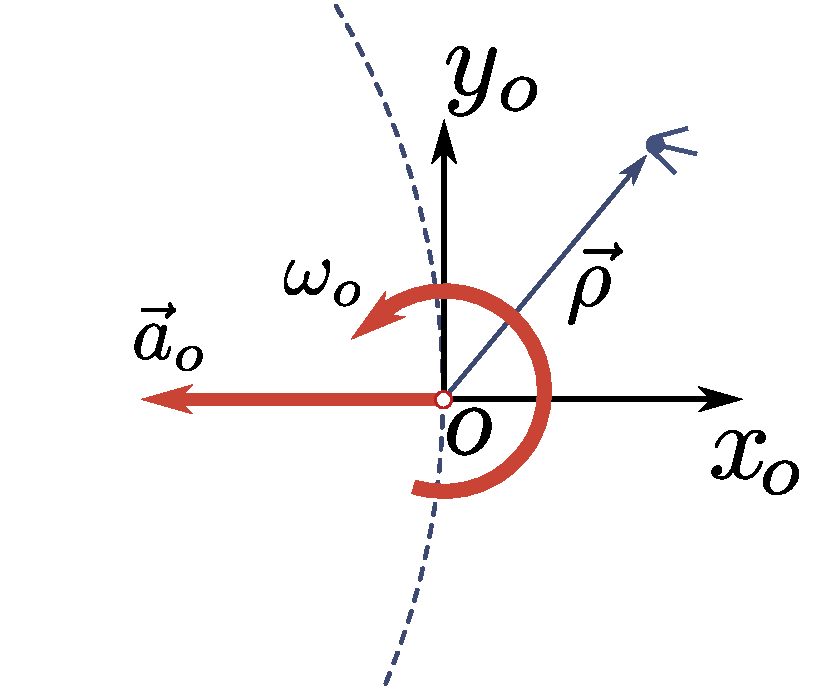
\includegraphics[width=0.95\textwidth]{non-inertial.pdf}
\end{figure}
\column{0.6\linewidth}
Система координат $Ox_0y_0z_0$ вращается с угловой скоростью $\omega_o$  вокруг оси $Oz_o$
\begin{equation}
  \boxed{\omega_o = \sqrt{\frac{\mu}{r_o^3}}}
\end{equation}
Начало системы координат  $Ox_0y_0z_0$  движется с ускорением
\begin{equation}
\boxed{a_o=\omega_o^2 r_o=\frac{V_o^2}{r_o}}
\end{equation}
\end{columns}
}



\frame{
\frametitle{Силы}
\begin{equation}
  \boxed{m \ddot{\vec \rho} = \vec F + \vec F_e  + \vec F_c}
\end{equation}
\begin{itemize}
 \item $\vec F_e$ -- переносная сила инерции:
\begin{equation}
  \vec F_e = - m \vec a_e = - m (\vec a_o + \vec \omega_o \times (\vec \omega_o \times \vec \rho))
\end{equation}
 \item $\vec F_c$ -- сила инерции Кориолиса:
\begin{equation}
  \vec F_c = - m \vec a_c =  - 2 m \, \vec \omega_o \times \dot{\vec \rho}
\end{equation}
 \item $\vec F$ -- гравитационная сила.
\end{itemize}
}

\frame
{
\frametitle{Переносная сила инерции}
\begin{columns}
\column{0.4\linewidth}
\begin{center}
 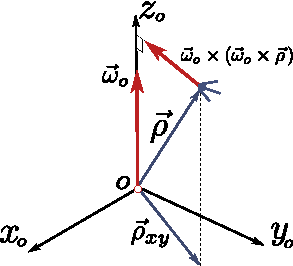
\includegraphics[width=1\linewidth]{./rho-rhop.pdf}
\end{center}
\column{0.6\linewidth}
\begin{multline}
\vec F_e = - m \vec{a}_e = \\ = - m [\vec a_o + \vec{\omega}_o \times (\vec{\omega}_o \times {\vec \rho}\,)]
\end{multline}
Центростремительно ускорение направлено к оси $Oz_0$
\begin{align*}
  & \vec a_o = - \omega_o^2 \vec r_o \\
  & \vec{\omega}_o \times (\vec{\omega}_o \times {\vec \rho}) = - \omega_o^2 \vec \rho_{xy}
\end{align*}
\begin{equation}
\boxed{\vec F_e = m (\omega_o^2 \vec r_o + \omega_o^2 \vec \rho_{xy})}
\end{equation}
\end{columns}
}


\frame{
\frametitle{Гравитационная сила}
\begin{equation}
  \boxed{m \ddot{\vec \rho} = \alert{\vec F} + \vec F_e  + \vec F_c}
\end{equation}
Гравитационная сила, действующая на КА
\begin{equation}
  \vec F = - G \frac{M_\Earth m}{|\vec r\,|^2} \cdot \frac{\vec r}{|\vec r\,|} = - \mu \frac{m}{|\vec r\,|^2} \cdot \frac{\vec r}{|\vec r \,|}
\end{equation}
\begin{equation}
  \boxed{\vec F = - \mu \frac{m}{|\vec r\,|^2} \cdot \frac{\vec r}{|\vec r\,|} = - \mu \frac{m \, \vec r}{|\vec r\,|^3}}
\end{equation}
}

\frame{
\frametitle{Уравнение движения}
После подстановки выражения, полученного для $\mu$ в выражение для гравитационной силы, действующий на КА 
\begin{equation}
 \vec F = - \mu \frac{m \, \vec r}{|\vec r\,|^3}  = - \omega_o^2 \left(\frac{r_o}{r}\right)^3 m \vec r
\end{equation}
уравнение относительного движения КА принимает вид
\begin{equation}
  m \ddot{\vec \rho} = - \omega_o^2 \left(\frac{r_o}{r}\right)^3 m \vec r + m \, \omega_o^2 ( \vec r_o + \vec \rho_{xy})  - 2 m \, \vec \omega_o \times \dot{\vec \rho}
\end{equation}
или
\begin{equation}\label{eq:eq2}
  \boxed{\ddot{\vec \rho} = - \omega_o^2 \alert{\left(\frac{r_o}{r}\right)^3} (\vec r_o+\vec \rho \,) + \omega_o^2 ( \vec r_o + \vec \rho_{xy})  - 2 \, \vec \omega_o \times \dot{\vec \rho}}
\end{equation}
}

\frame{
\frametitle{Линеаризация $(r_o/r)^3$}
\begin{multline}
  \left(\frac{r_o}{r}\right)^3 = \left(\frac{r}{r_o}\right)^{-3} = \left[\left(\frac{r}{r_o}\right)^2\right]^{-\frac{3}{2}} = \left[\frac{(\vec r_o+\vec \rho \, )^2}{r_o^2}\right]^{-\frac{3}{2}} = \\ =
  \left[\frac{r_o^2 + 2 \, \vec r_o \cdot \vec \rho + \rho^2}{r_o^2}\right]^{-\frac{3}{2}} = \left(\frac{r_o^2 + 2 \, r_o x + \rho^2}{r_o^2}\right)^{-\frac{3}{2}} = \\
  = \left(1+ \frac{2x}{r_o} + \textcolor{gray}{ \frac{\rho^2}{r_o^2} } \right)^{-\frac{3}{2}}
\end{multline}
\begin{equation}
 \boxed{\left(\frac{r_o}{r}\right)^3 \approx \left(1+ \frac{2x}{r_o} \right)^{-\frac{3}{2}}}
\end{equation}
}


\frame{
\frametitle{Линеаризация $(r_o/r)^3$}
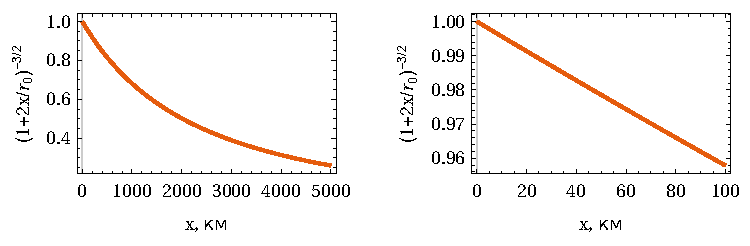
\includegraphics[width=1\linewidth]{f.pdf} 

Для $x \ll r_o$ выражение $(1+2x/r_0)^{-3/2}$ можно разложить в ряд по степеням $x$ в окрестности $x=0$, оставив только линейную часть разложения
\begin{equation}
 \left(1+ \frac{2x}{r_o} \right)^{-\frac{3}{2}} \approx 1 - 3\frac{x}{r_o}
\end{equation}
}


\frame{
\frametitle{Линеаризованное уравнение движения}
Исходное уравнение относительного движения (нелинейное)
\begin{equation}\label{eq:eq2}
  \boxed{\ddot{\vec \rho} = - \omega_o^2 \alert{\left(\frac{r_o}{r}\right)^3} (\vec r_o+\vec \rho \,) + \omega_o^2 ( \vec r_o + \vec \rho_{xy})  - 2 \, \vec \omega_o \times \dot{\vec \rho}}
\end{equation}
Линеаризованное уравнение
\begin{multline}
  \ddot{\vec \rho} = - \omega_o^2 \alert{\left(1 - 3\frac{x}{r_o}\right)} \left(\vec r_o+\vec \rho \,\right) + \omega_o^2 ( \vec r_o + \vec \rho_{xy})  - 2 \, \vec \omega_o \times \dot{\vec \rho}_o
= \\ =
\underline{- \omega_o^2 \vec r_o} - \omega_o^2 \vec \rho + 3 \, \omega_o^2 \frac{x}{r_o} \vec r_o +  \textcolor{gray}{3 \, \omega_o^2 \frac{x}{r_o} \vec \rho} + \underline{\omega_o^2 \vec r_o} + \omega_o^2 \vec \rho_{xy} - 2 \, \vec \omega_o \times \dot{\vec \rho}_o
= \\ =
  3 \, \omega_o^2 \frac{x}{r_o} \vec r_o + \omega_o^2 (\vec \rho_{xy}-\vec \rho \,) - 2 \, \vec \omega_o \times \dot{\vec \rho}_o
\end{multline}
}


\frame{
\frametitle{Линеаризованное уравнение}
\begin{itemize}
 \item Векторное уравнение
\begin{equation}
  \boxed{\ddot{\vec \rho} = 3 \, \omega_o^2 \frac{x}{r_o} \vec r_o + \omega_o^2 (\vec \rho_{xy}-\vec \rho \,) - 2 \, \vec \omega_o \times \dot{\vec \rho}}
\end{equation}
 \item Уравнение в координатной форме, в системе координата $Ox_oy_oz_o$
\begin{equation}
  \begin{bmatrix} \ddot x \\ \ddot y \\ \ddot z \end{bmatrix} = 3 \, \omega_o^2 \frac{x}{r_o}
  \begin{bmatrix} r_o \\ 0 \\ 0 \end{bmatrix} +
  \omega_o^2 \begin{bmatrix} 0 \\ 0 \\ -z \end{bmatrix} -
  2 \begin{bmatrix} \vec i & \vec j & \vec k \\ 0 & 0 & \omega_o \\ \dot x & \dot y & \dot z \end{bmatrix}
\end{equation}
\end{itemize}
}

\frame{
\frametitle{Линеаризованные уравнения}
Система дифференциальных уравнений:
\begin{equation}
\left\{
\begin{array}{l}
  \ddot x = 3 \, \omega_o^2 x + 2 \omega_o \dot y, \\
  \ddot y = - 2 \, \omega_o \dot x, \\
  \ddot z = - \omega_o^2 z.
\end{array}
\right.
\end{equation}
Начальные условия:
\begin{equation}\label{eq:nu}
\begin{array}{ll}
  x(0) = x_0, & \dot x(0) = \Delta V_x \\
  y(0) = y_0, & \dot y(0) = \Delta V_y \\
  z(0) = z_0, & \dot z(0) = \Delta V_z  
\end{array}
\end{equation}
}

\section{Интегрирование уравнений движения}

\frame{
\frametitle{Уравнение 3}
\begin{itemize}
 \item Движение вдоль оси $z$ независимо от движений вдоль осей $x$ и $z$
$$
  \boxed{\ddot z + \omega_o^2 z = 0}
$$
 \item Вид решения
$$
  z(t) = C_1 \sin \omega_o t + C_2 \cos \omega_o t
$$
 \item С учётом начальных условий
$$
  z(0) = C_2, \; \dot z(0) = \Delta V_z = C_1 \omega_o
$$
\begin{equation}
  \boxed{z(t) =  \frac{\Delta V_z}{\omega_o} \sin \omega_o t + z_0 \cos \omega_o t }
\end{equation}
\end{itemize}
}


\frame{
\frametitle{Уравнение 2}

\begin{equation}\label{eq:ddy}
  \ddot y = - 2 \, \omega_o \dot x
\end{equation}
Введем обозначение $u_y = \dot y $ и проинтегрируем уравнение \eqref{eq:ddy}
$$
  \int_{\Delta V_y}^{u_y} du_y = - 2 \, \omega_o \int_{x_{0}}^{x} dx
  \quad \rightarrow \quad
  u_y - \Delta V_y = - 2 \, \omega_o (x - x_0)
$$
\begin{equation}
  \boxed{\dot y = \Delta V_y - 2 \, \omega_o (x - x_0)}
\end{equation}
}

\frame{
\frametitle{Уравнение 1}
После подстановки решения
$$
\dot y = \Delta V_y - 2 \, \omega_o (x - x_0)
$$
в первое уравнение системы
$$
  \ddot x = 3 \, \omega_o^2 x + 2 \omega_o \dot y
$$
уравнение движения вдоль оси $x$ принимает вид
\begin{equation}
  \ddot x + \omega_o^2 x = 2 \omega_o \Delta V_y + 4 \, \omega_o^2 x_0
\end{equation}
}

\frame{
\frametitle{Уравнение 1}
Неоднородное линейное дифференциальное уравнение
$$
  \ddot x + \omega_o^2 x = 2 \omega_o \Delta V_y + 4 \, \omega_o^2 x_0
$$
Вид решения
$$
  x(t) = C_3 \sin \omega_o t +  C_4 \cos \omega_o t + C_5
$$
где $C_5$ -- частное решение неоднородного дифференциального уравнения
\begin{equation}
 \boxed{C_5 = \frac{2 \, \omega_o \Delta V_y + 4 \, \omega_o^2 x_0}{\omega_o^2} = \frac{2 \Delta V_y}{\omega_o} + 4 \, x_0}
\end{equation}
}

\frame{
\frametitle{Уравнение 1}
Неоднородное линейное дифференциальное уравнение
$$
  \ddot x + \omega_o^2 x = 2 \omega_o \Delta V_y + 4 \, \omega_o^2 x_0
$$
Вид решения
$$
  x(t) = C_3 \sin \omega_o t +  C_4 \cos \omega_o t + C_5
$$
Постоянные интегрирования $C_3$, $C_4$  определяются из начальных условий
\begin{equation}
  x(0) = x_0 = C_4 + C_5\; \rightarrow \boxed{C_4 = -\frac{2 \Delta V_y}{\omega_o} - 3 \, x_0}
\end{equation}
\begin{equation}
  \dot x(0) = \Delta V_x = C_3 \omega_o \; \rightarrow \boxed{C_3 = \frac{\Delta V_x}{\omega_o}}
\end{equation}
}

\frame{
\frametitle{Уравнение 1}
После подстановки решения первого уравнения (для оси $x_0$)
$$
  \boxed{x(t) = \frac{\Delta V_x}{\omega_o} \sin \omega_o t - \left(\frac{2 \Delta V_y}{\omega_o} + 3 \, x_0\right) \cos \omega_o t + \frac{2 \Delta V_y}{\omega_o} + 4 \, x_0}
$$
во второе уравнение
$$
  \dot y = \Delta V_y - 2 \, \omega_o (x - x_0)
$$
$$
  \dot y = - 2 \, \omega_o \left(  \frac{\Delta V_x}{\omega_o} \sin \omega_o t - \left(\frac{2 \Delta V_y}{\omega_o} + 3 \, x_0\right) \cos \omega_o t \right ) - 3 \, \Delta V_y - 6 \, \omega_o \, x_0
$$
и интегрирования
\small
$$
  \boxed{y = y_0 + 2 \, \frac{\Delta V_x}{\omega_o} \left( \cos \omega_o t - 1 \right)
+ \left(4 \, \frac{\Delta V_y}{\omega_o} + 6 \, x_0 \right)\sin \omega_o t - (6 \, \omega_o \, x_0 + 3 \, \Delta V_y) t }
$$
}

\frame{
\frametitle{Уравнения относительного движения}
\small
\begin{align*}
  & x(t) = \frac{\Delta V_x}{\omega_o} \sin \omega_o t - \left(\frac{2 \Delta V_y}{\omega_o} + 3 \, x_0\right) \cos \omega_o t + \frac{2 \Delta V_y}{\omega_o} + 4 \, x_0 \\
  & y(t) = y_0 + 2 \, \frac{\Delta V_x}{\omega_o} \left( \cos \omega_o t - 1 \right)
+ \left(4 \, \frac{\Delta V_y}{\omega_o} + 6 \, x_0 \right)\sin \omega_o t - (6 \, \omega_o \, x_0 + 3 \, \Delta V_y) t \\
  & z(t) =  \frac{\Delta V_z}{\omega_o} \sin \omega_o t + z_0 \cos \omega_o t
\end{align*}
}

\frame{
\frametitle{Уравнения относительного движения}
Для случая $x_0=y_0=z_0=0$
\begin{align*}
  & x(t) = \frac{\Delta V_x}{\omega_o} \sin \omega_o t - \frac{2 \Delta V_y}{\omega_o} \cos \omega_o t + \frac{2 \Delta V_y}{\omega_o}\\
  & y(t) = 2 \, \frac{\Delta V_x}{\omega_o} \left( \cos \omega_o t - 1 \right)
+ 4 \, \frac{\Delta V_y}{\omega_o} \sin \omega_o t - 3  \Delta V_y t \\
  & z(t) =  \frac{\Delta V_z}{\omega_o} \sin \omega_o t
\end{align*}
}


{
\usebackgroundtemplate{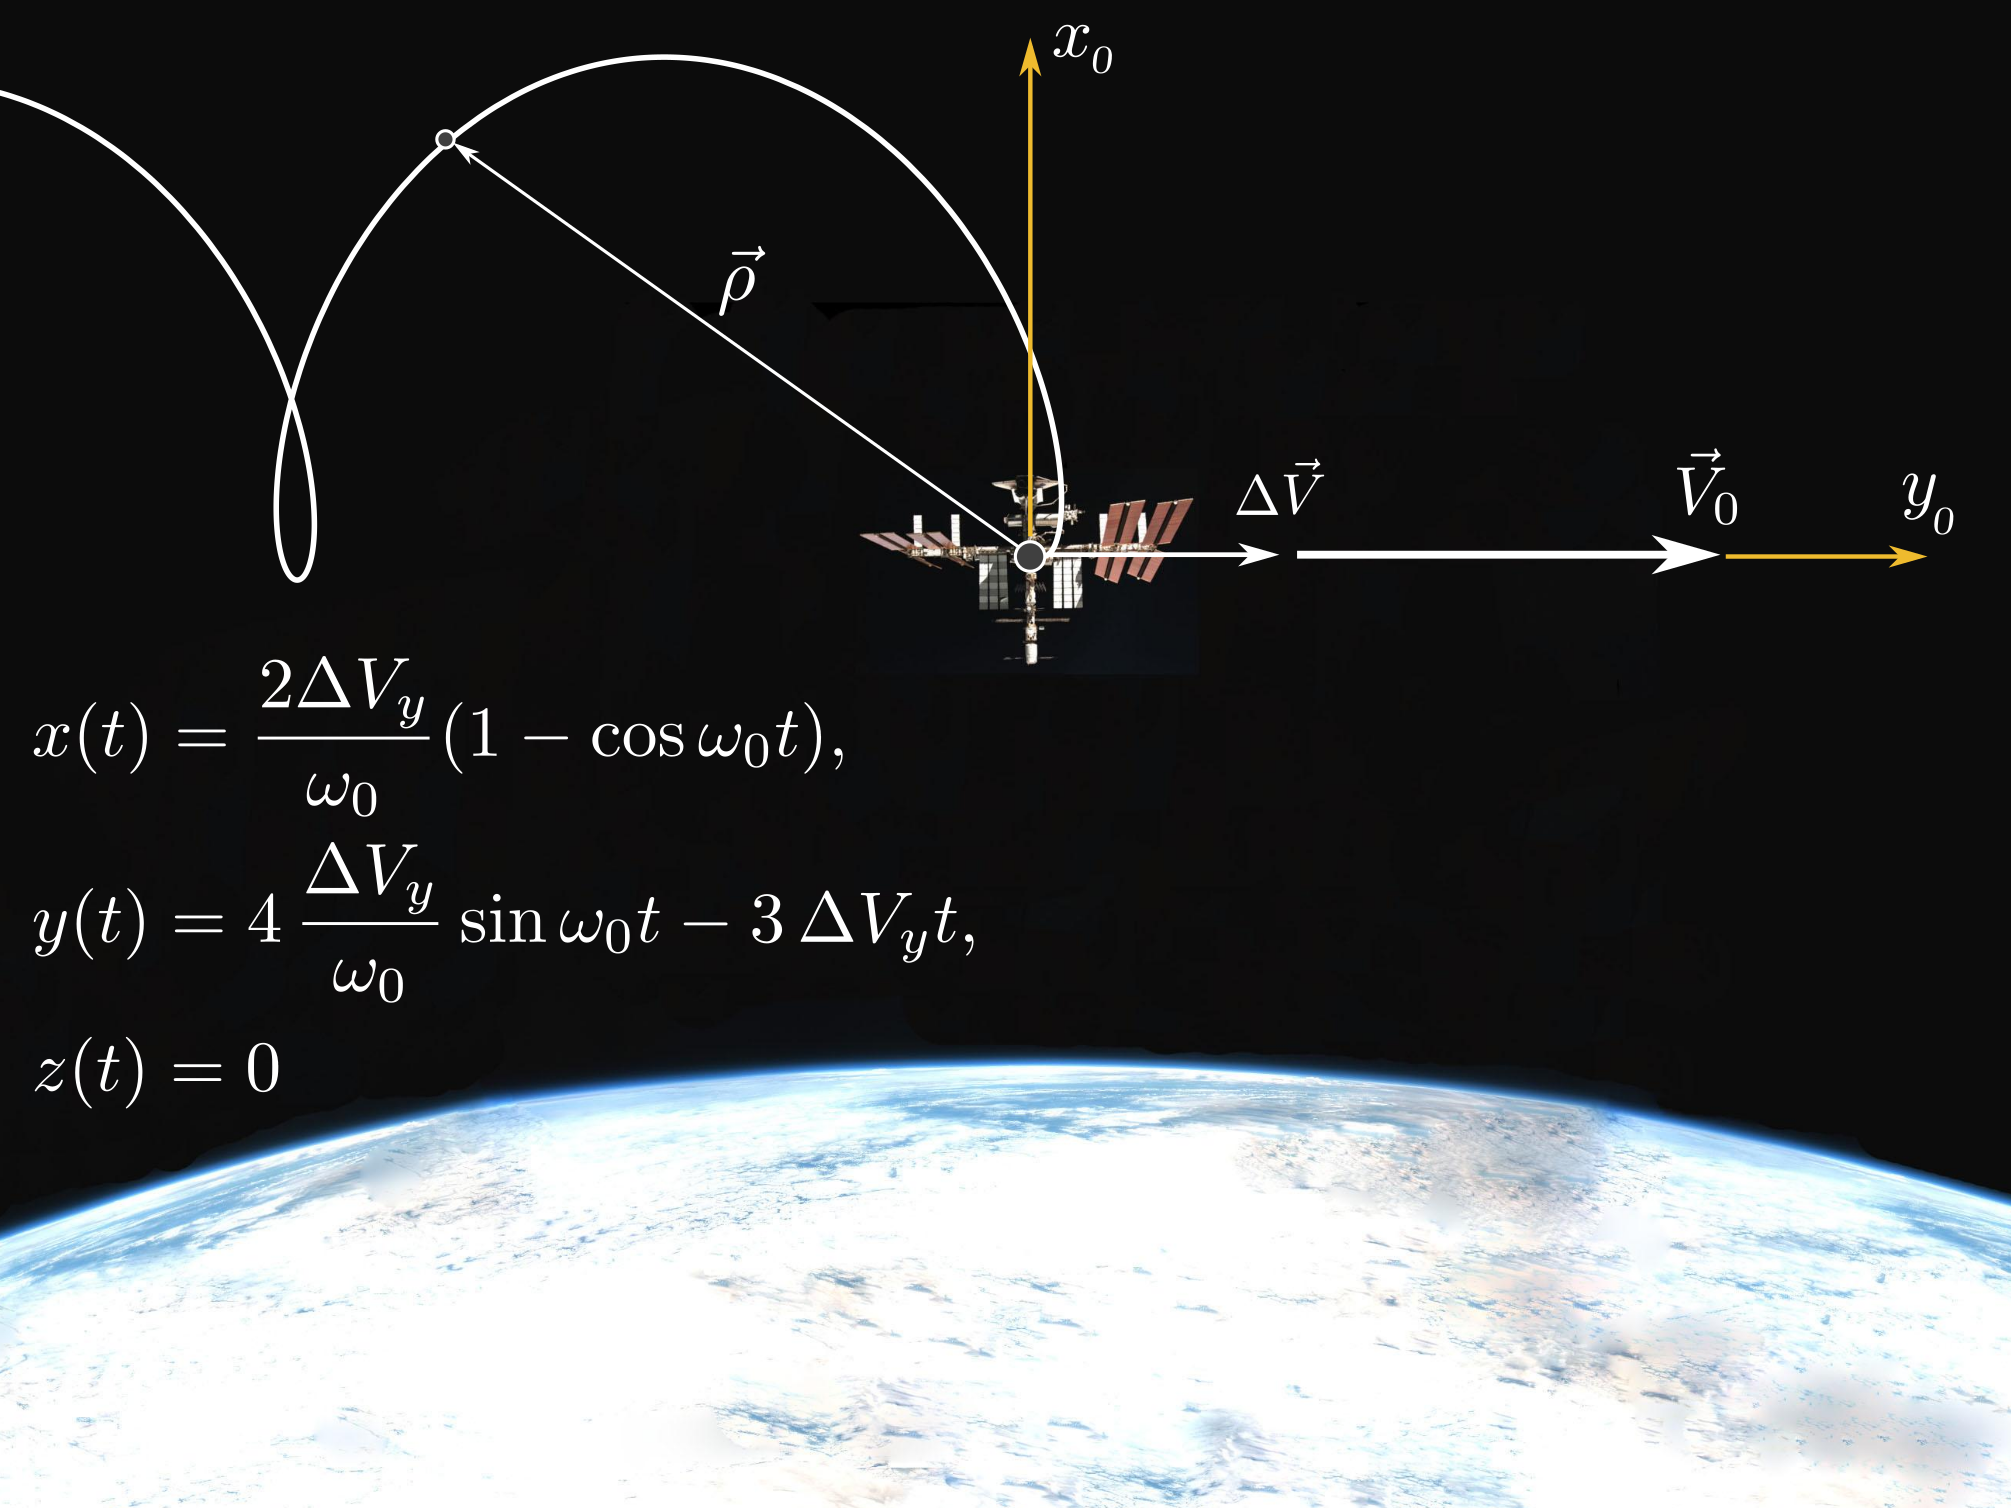
\includegraphics[width=\paperwidth,height=\paperheight]{./dV_forward.png}}
\begin{frame}[plain]
\end{frame}
}

{
\usebackgroundtemplate{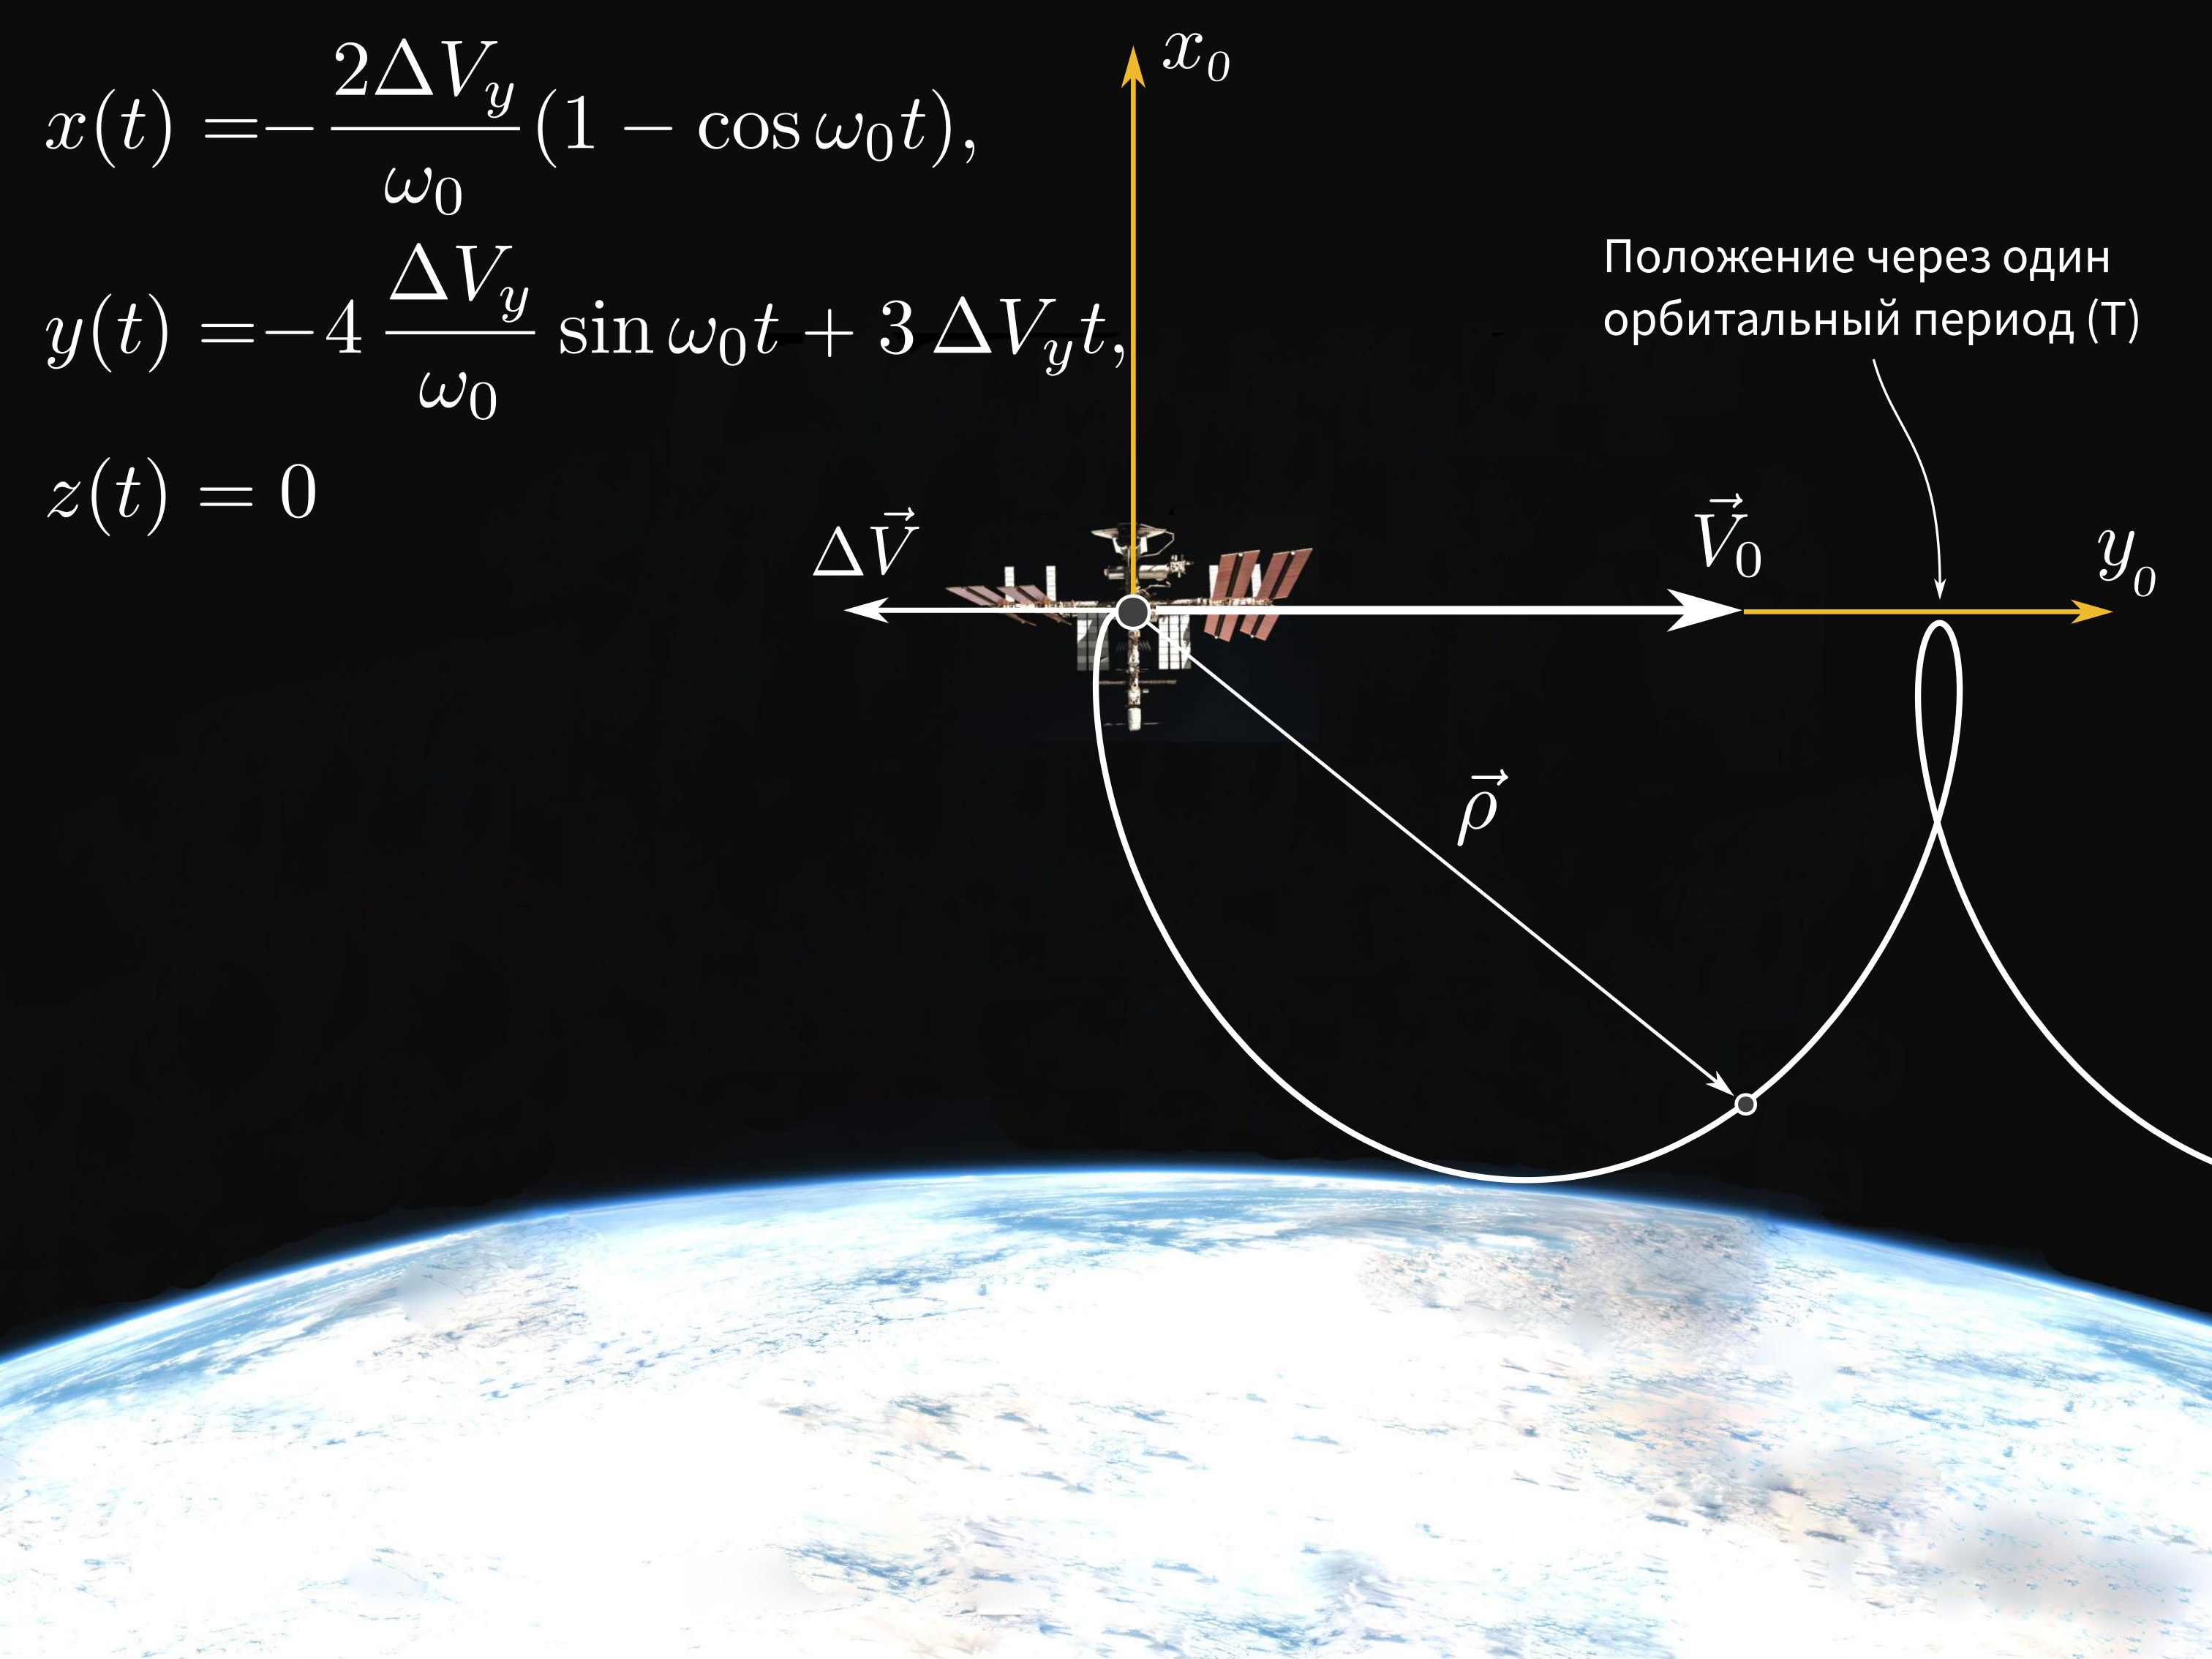
\includegraphics[width=\paperwidth,height=\paperheight]{./dV_back.png}}
\begin{frame}[plain]
\end{frame}
}


{
\usebackgroundtemplate{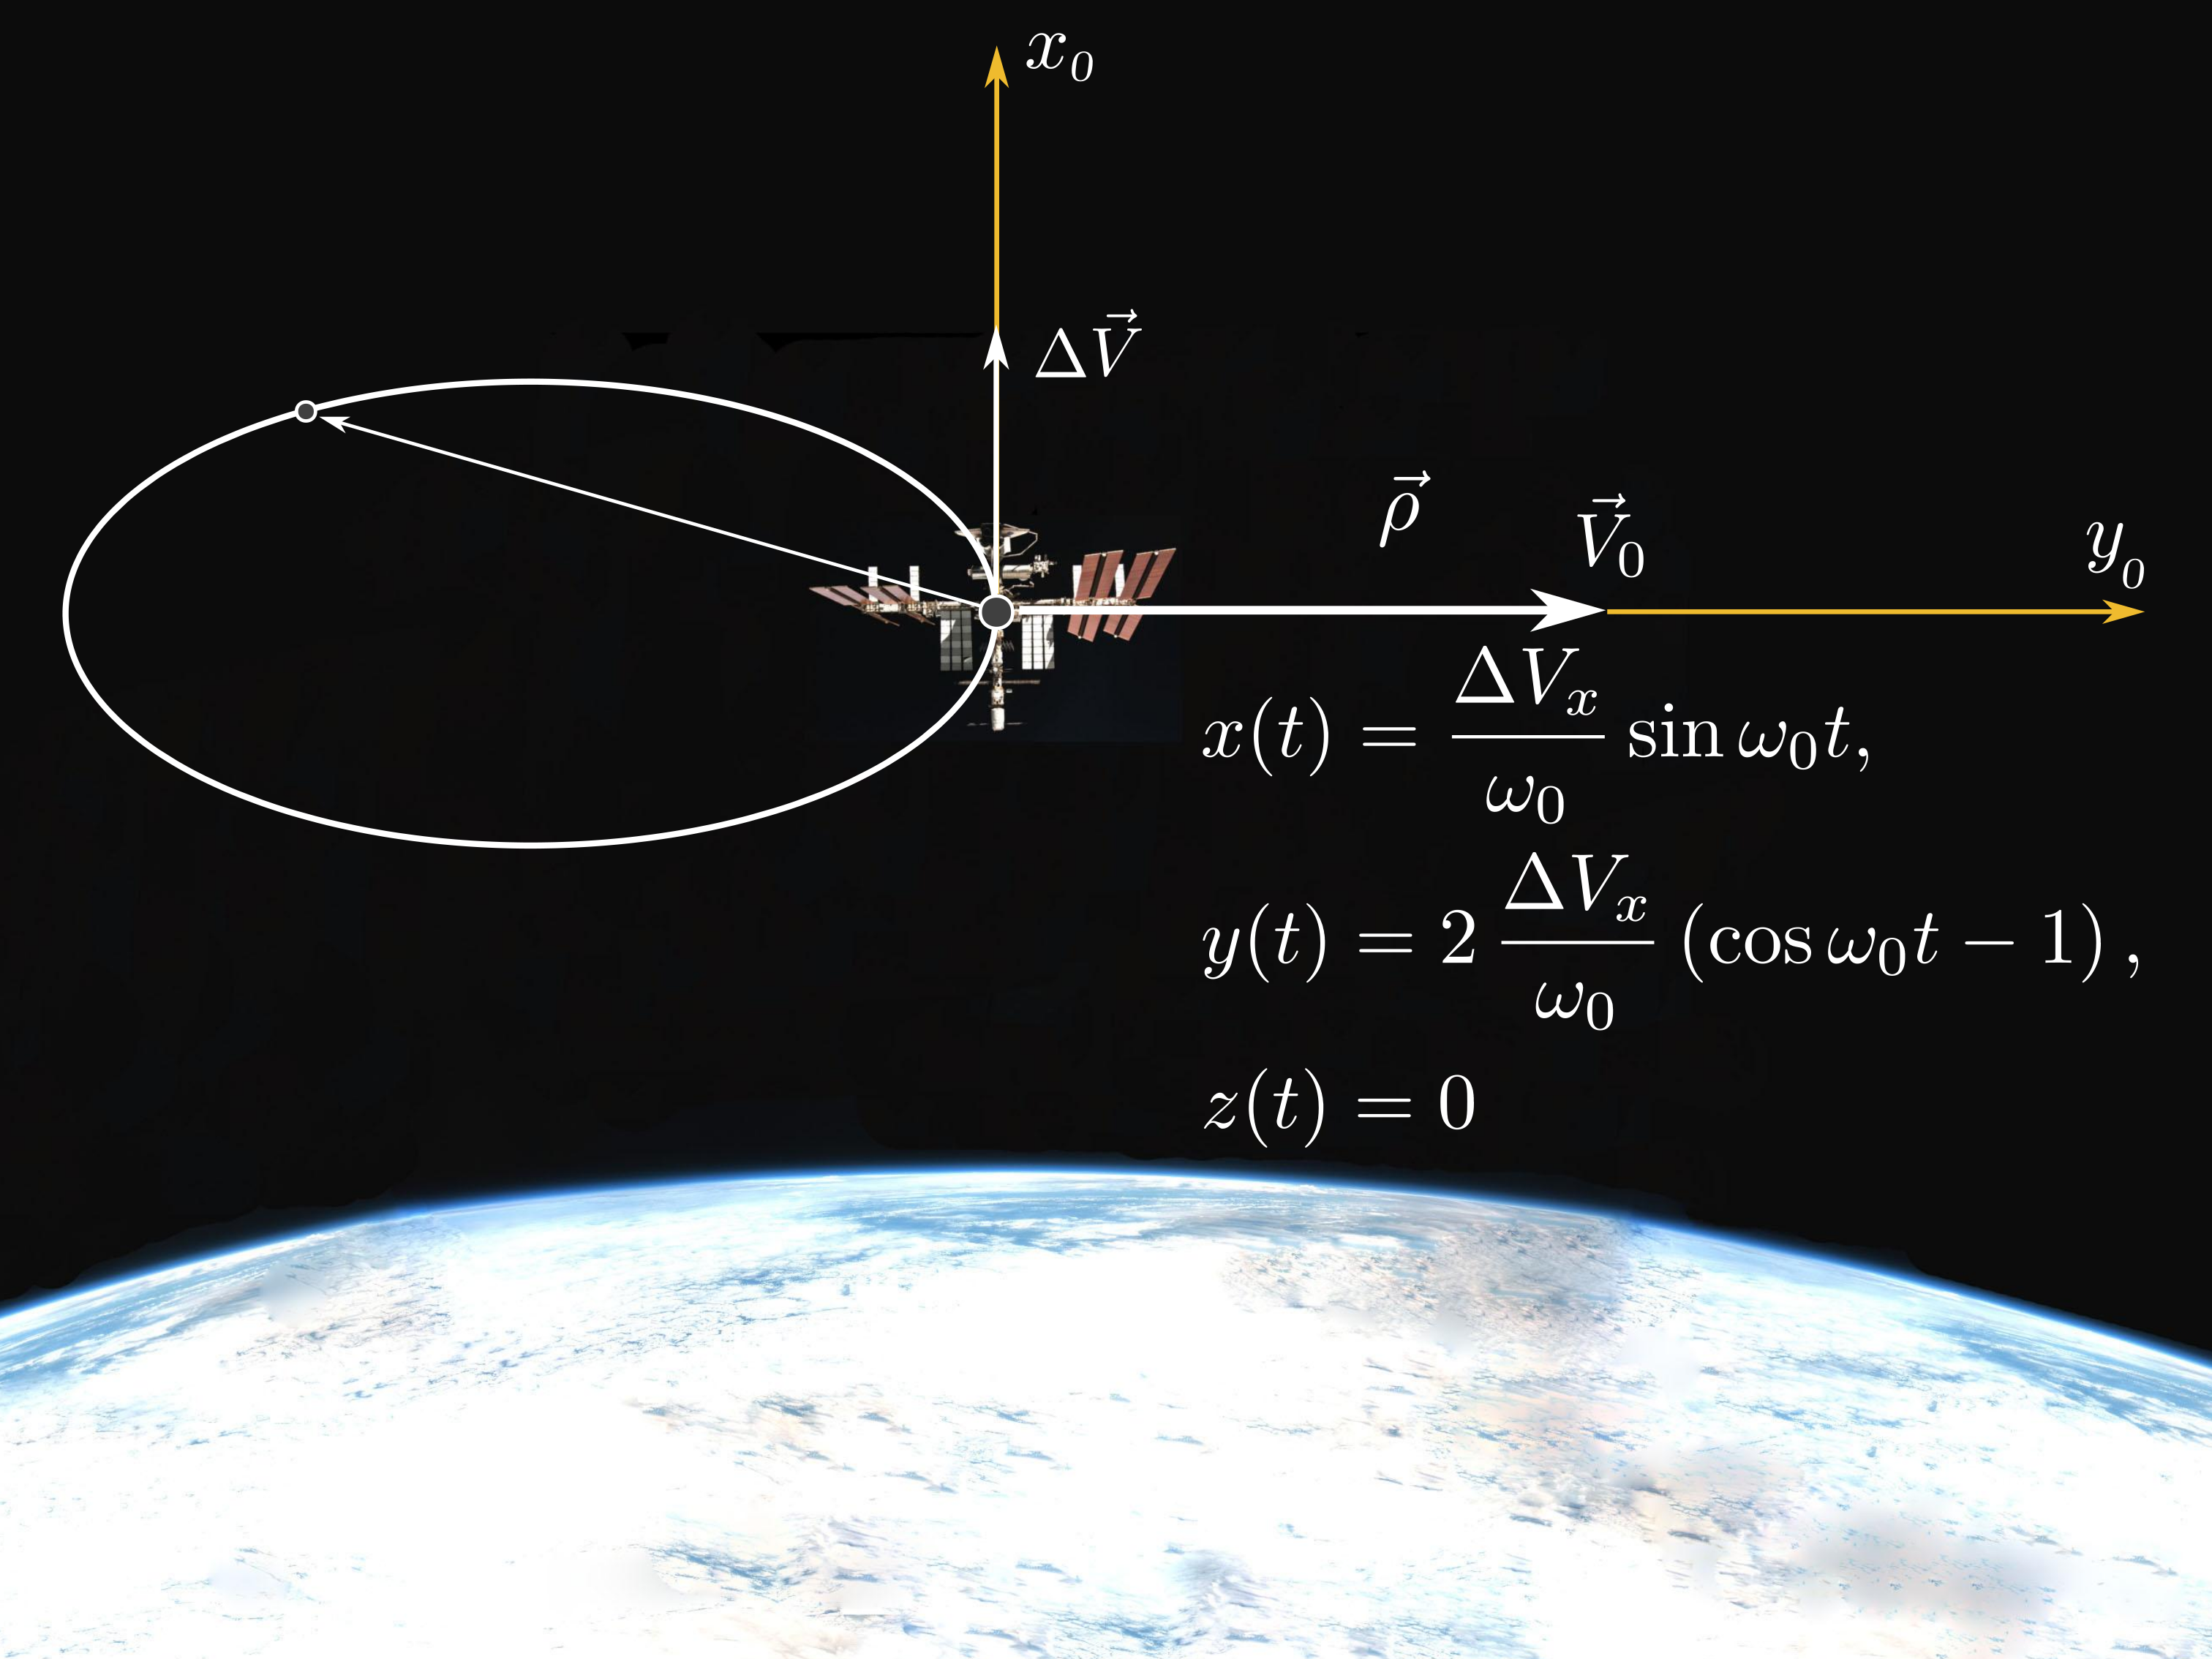
\includegraphics[width=\paperwidth,height=\paperheight]{./dV_up.png}}
\begin{frame}[plain]
\end{frame}
}

\frame{
\frametitle{Отделение по нормали к орбите}
\begin{columns}
\column{0.45\linewidth}
\begin{figure}[htbp]
  \centering
  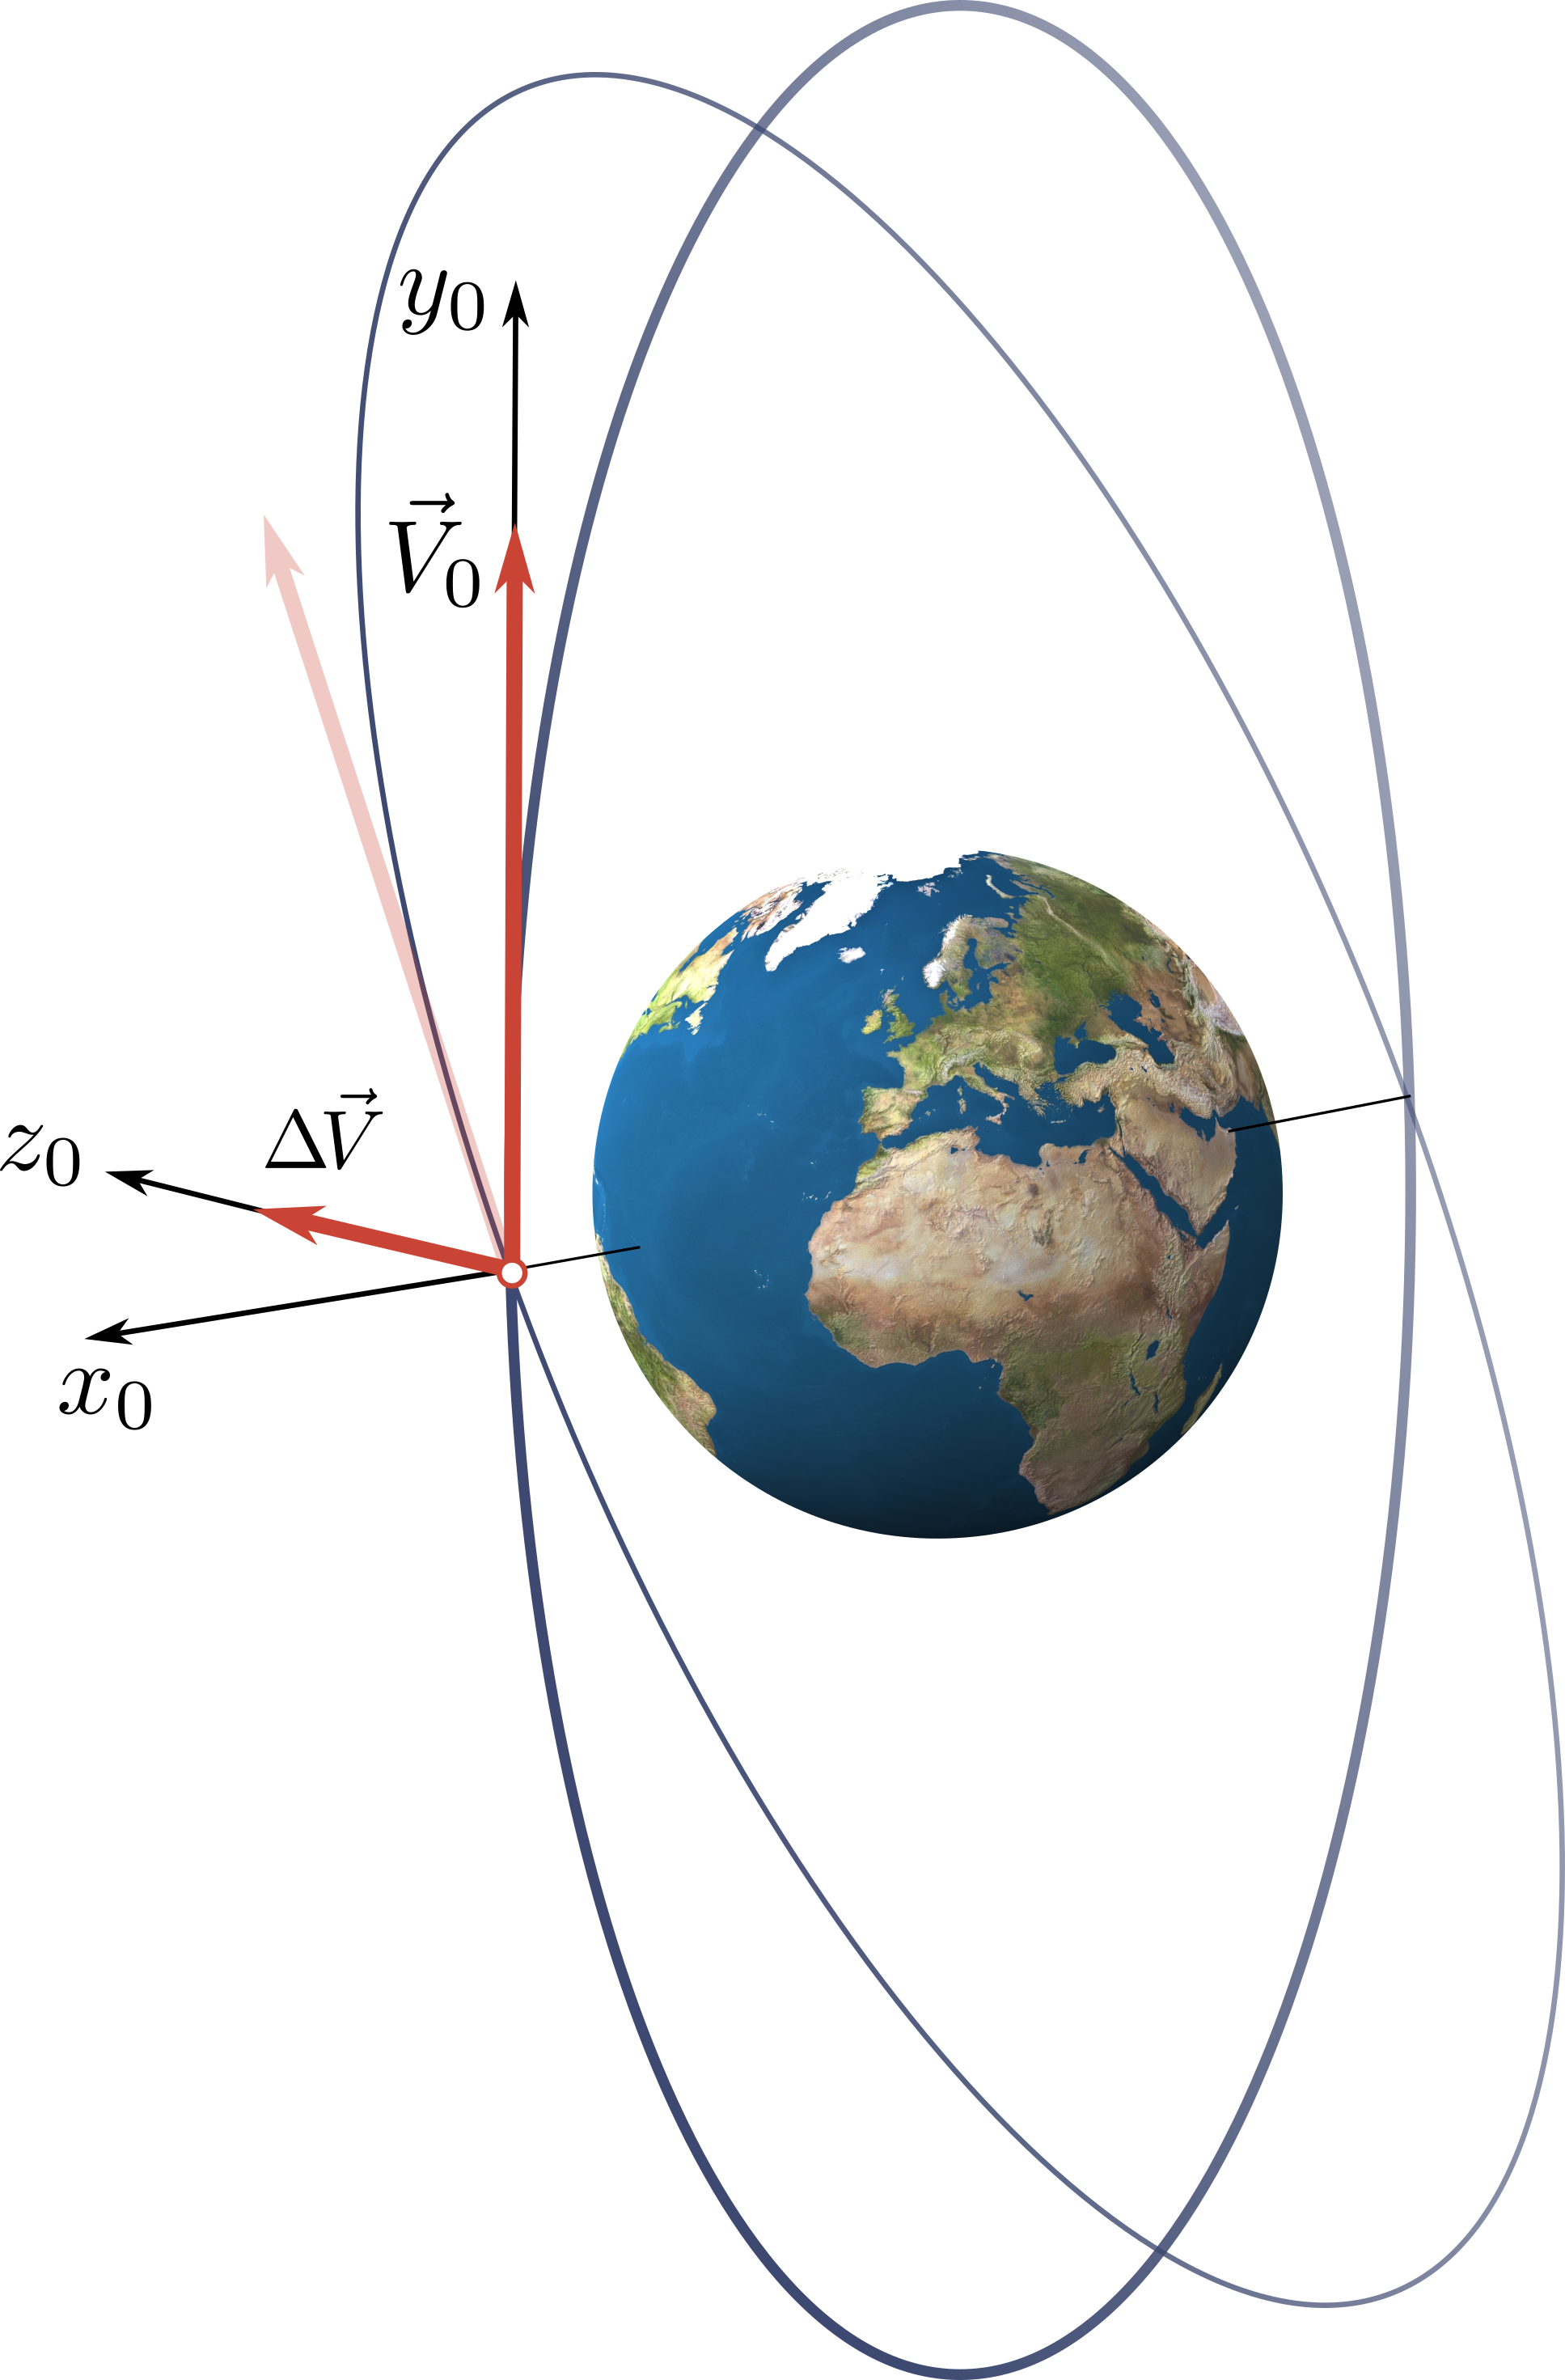
\includegraphics[width=1\textwidth]{dV_side.png}
\end{figure}
\column{0.55\linewidth}
$$
\Delta V_x=\Delta V_y=0, \Delta V_z \neq 0
$$
\begin{align*}
  & x(t) = 0, \\
  & y(t) = 0, \\
  & z(t) =  \frac{\Delta V_z}{\omega_0} \sin \omega_0 t
\end{align*}
\end{columns}
}

\frame{
\frametitle{Выводы}
\begin{itemize}
 \item Объект, отделившийся от станции вдоль нормали к плоскости орбиты, вернётся на станцию через половину орбитального периода станции.
 \item Объект, отделившийся от станции вдоль её радиус-вектора, возвратится на станцию через орбитальный период.
 \item Если вектор приращения объекта относительно станции направлен вдоль вектора её орбитальной скорости, то с каждым орбитальным периодом расстояние между объектом и станцией будет увеличиваться.
\end{itemize}
}

\section{Задание}

\begin{frame}[fragile]{Групповое отделение КА}
  \begin{center}
    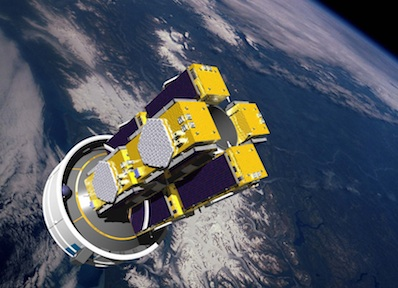
\includegraphics[width=0.8\linewidth]{ariane_galileo.jpg} 
  \end{center}
  \tiny{EADS Astrium}
\end{frame}


\begin{frame}[fragile]{Групповое отделение КА}
  \begin{center}
    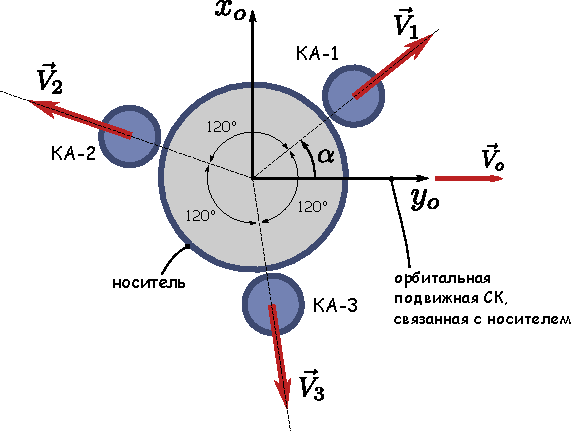
\includegraphics[width=0.9\linewidth]{./3KA.pdf} 
  \end{center}
\end{frame}


\begin{frame}[fragile]{Групповое отделение КА}
От носителя (орбитальной ступени) одновременно отделяется три малых космических аппарата с одинаковыи скоростями $V_1 = V_2 = V_3$ = 1  м/с. Векторы приращений скоростей малых КА относительно орбитальной ступени лежат в плоскости орбиты, как показано на рисунке на предыдущем слайде. Носитель движется по круговой орбите высотой 300 км.
\end{frame}

\begin{frame}[fragile]{Групповое отделение КА}
   \begin{enumerate}
   \item Используя уравнения относительного орбитального движения, определите наилучший угол отделения КА -- $\alpha$, при котором минимальное расстояние между любыми КА и между любым КА и носителем через один орбитальный период носителя было бы максимальным. 
   \item Постройте траектории движения КА относительно носителя (на одном рисунке).
   \item Постройте графики изменения расстояний между КА и носителем и между каждой парой КА (на одном рисунке).
  \end{enumerate}
  \end{frame}
 
\end{document}
